\documentclass[../ode.tex]{subfiles}
\begin{document}
    \chapter{\sffamily The Basics}

    \section{\sffamily Antiderivatives}
    Solving an integral like $x(t) = \int g(t) \mathop{\mathrm{d}t} $ is the problem of finding the function $x(t)$ such that its
    derivative is equal to $g(t)$ i.e. it holds that:
    \begin{equation*}
        x(t) = \int g(t) \mathop{\mathrm{d}t} \iff x' = g(t)    
    \end{equation*}
    So, for solving an equation of type $x' = g(t)$ i.e. the derivative of the solution is a function only of the independent
    variable $t$, we just have to integrate the function $g(t)$ to obtain the solution.

    \hfill
    \begin{thm}{Fundamental Theorem of Calculus}{a}
        If $g(t)$ is a continuos function then:
        \begin{equation}\label{funthcal}
            \mathrm{D}_{t} \int_{a}^{t} g(s) \mathop{\mathrm{d}s} = g(t)
        \end{equation}
    \end{thm}
    That means that the function 
    \begin{equation*}
        G(s) = \int_{a}^{t} g(s) \mathop{\mathrm{d}s} 
    \end{equation*}
    is an antiderivative. 
    \subsubsection{\sffamily Functions defined from integrals}
    This definition of antiderivative let's us define some special functions as solutions to certain derivatives. Perhaps the most
    common example is the logarithm funtion. It can be defined as:
    \begin{equation*}
        \ln(t) = \int_{1}^{t} \frac{1}{s}\mathop{\mathrm{d}s} , \quad t>0
    \end{equation*}
    Or, equivalently, as a DE:
    \begin{equation*}
        x' = \frac{1}{t}, \quad x(1) = 0 
    \end{equation*}
    Defines the logarithm function.

    Another useful function defined as a solution to a integral is the \emph{error function}. It is defined as:
    \begin{equation*}
        \mathrm{erf}(t) = \frac{2}{\sqrt{\pi}} \int_{0}^{t} \mathrm{e}^{-s ^{2}}\mathop{\mathrm{d}s}
    \end{equation*}
    This integral is of most use in statistics and diffusion problems.

    \section{\sffamily Separable equations}
    I don't really get (nor find) the formal aproach to the derivation of this method without the use (or misuse) of the
    $\frac{\mathop{\mathrm{d}x}}{\mathop{\mathrm{d}t}}$ notation . So I will use it as a black box.
    
    \begin{prop}{Solving Separable equations}{a}
        If an equation can be written as:
        \begin{equation*}
            x' = f(x)g(t)
        \end{equation*}
        It can be solved as
        \begin{equation*}
            x' = f(x)g(t) \iff \int \frac{1}{f(x)}\mathop{\mathrm{d}x} = \int g(t) \mathop{\mathrm{d}t}
        \end{equation*}
        This gives the \emph{implicit} solution to the DE. If we can then solve for $x$ we'll have the \emph{explicit} solution.
    \end{prop}
    \section{\sffamily Linear equations}
    A DE of the form:
    \begin{equation*}
        x' + p(t)x = q(t)
    \end{equation*}
    is called a \emph{first order linear equation}. If a first order equation can not be put into this form its then called a 
    first order \emph{nonlinear} equation. Some terminology:
    
    \begin{itemize}
        \item The function $q(t)$ is called the \emph{forcing} or \emph{source term}
        \item The form with $q(t) \neq 0$, is called the \emph{normal form}.
        \item When $q(t) = 0$ then in called the \emph{homogeneous form}
    \end{itemize}    

    This kind of equation have a nice property: the LHS of the equation can be multiplied by a function $\mu = \mu(t)$ that
    transforms it into a total derivative i.e.:
    \begin{equation*}
        \mu(t)(x' + p(t)x) = (\mu(t)x)'     
    \end{equation*}
    Such a function is called \emph{integrating factor} and is given by:
    \begin{equation*}
        \mu(t) = \exp\left(\int p(t) \mathop{\mathrm{d}t}\right) = \mathrm{e}^{P(t)};\quad P(t) = \int p(t) \mathop{\mathrm{d}t}
    \end{equation*}

    \begin{prop}{Solving First Order Linear Equations}{b}
        \begin{enumerate}
            \item Multiply both sides by the integrating factor. With this we obtain a simple DE:
                \begin{equation*}
                    x' + p(t)x = q(t) \implies  \mu(x' + px) = (\mu x)' \iff(\mathrm{e}^{P(t)} x)' = \mathrm{e}^{P(t)}q(t)
                \end{equation*}
            \item And this equation defines the integral:
                \begin{equation*}
                    \mathrm{e}^{P(t)} x = \int \mathrm{e}^{P(t)} q(t) \mathop{\mathrm{d}t} + C
                \end{equation*}
                
            \item And the solution is the obtained multiplying both sides by $\mathrm{e}^{-P(t)} $ :
                \begin{equation*}
                    \boxed{x(t) = \mathrm{e}^{-P(t)} \int \mathrm{e}^{P(t)} q(t) \mathop{\mathrm{d}t} + C \mathrm{e}^{-P(t)}}
                \end{equation*}
        \end{enumerate}
    \end{prop}
    
    \begin{thm}{Structure Theorem}{struct}
        The general solution of the linear DE $x' + p(t)x = q(t)$ can be expressed in the form: 
        \begin{equation*}
            x(t) = x_{h}(t) + x_{p}(t)
        \end{equation*}
        
        Where $x_{h}(t)$ is the solution to the \emph{homogeneous} equation, and $x_{p}(t)$ is the solution to one nonhomonegeous
        equation:
        \begin{equation*}
            x_{h}(t) = C \mathrm{e}^{P(t)}, \quad x_{p}(t)=\mathrm{e}^{-P(t)} \int q(t) \mathrm{e}^{P(t)} \diff t ; \quad
            P(t)=\int p(t)\diff t
        \end{equation*}

        Both function receive a special name in the applied math world: $x_{h}(t)$ is called the \emph{transient solution}, as it
        envolves the initial condition. And $x_{p}(t)$ is the so called \emph{steady state solution}.
    \end{thm}

    
    \section{\sffamily One-Dimensional Dynamical Systems}
    Many aplications lead to differential equations that have no \emph{explicit} dependence in time i.e. the change $x'(t)$ only
    dependends on the state itself $x = x(t)$.
   
    Such equation have the form:
    \begin{equation*}
        x' = f(x) 
    \end{equation*}
    They do not have a \emph{explicit} dependence of $t$, but remember that $x$ does depend of time. 

    This type of equations receive the name of \emph{autonomous}. The common way of representing the solution to a DE is to plot
    $x$ vs $t$ in the $tx$ plane. But here we'll interpret a solution as a  \emph{state} $x$ moving along a one-dimensional line
    i.e. the $x$ axis. The $x$ axis is a state space called the \emph{phase line}.

    \subsection{\sffamily Autonomous Equations}
    
    In animal populations, the number of specimens does not follow a exponential grow. That is because the all the population has
    to compete for a limited number or resources, so the increase in population decreases as the number in specimens grow i.e. $x'$ 
    decreases as $x$ increases. The simplest assumption is that the relative growth rate ($\frac{x'}{x}$ drecreases linearly as
    the  population increases, and the rate becomes zero at some maximum \emph{carrying capacity} $K$. This is called the
    \emph{logistic model}  of population growth.
    \begin{equation*}
        \frac{x'}{x} = r(1-\frac{x}{K}) \quad \text{or}  \quad x' = r(1-\frac{x}{K})x\quad \text{or}  \quad 
        x' = rx - \frac{r}{K}x ^{2}
    \end{equation*}
    And note that it is an autonomous equation. In the last equation the first term is the \emph{growth term}. The second term,
    which is a negative quadratic in $x$, is the \emph{competition term}. 

    We note that this equation has two constant solutions: $x(t) = 0$, $x(t)=K$. Corresponding to extinction and
    maximun animal capacity. These solutions are found by setting $x'=0$ as that forces $x= \text{constant} $. These constant
    solutions to autonomous equations are called \emph{steady-state} or \emph{equilibrium} solutions.

    It makes sense (and we can see it in the equations) that if $0<x<K$ the population tends to increase i.e. $x'>0$. And if  $x>K$ 
    i.e. there is an over-population, then $x'<0$; the population tends to decrease. All this information can be synthesized in
    the \emph{phase line}. 

    \subsection{\sffamily Phase Line}
    
    We indicate this trends by arrows in the equilibrium points. If the population in greater than $0$ and
    less than $K$ the population tends to $K$. If it's greater than $K$ then it also thends to $K$. 

    \begin{figure}[ht]
        \centering
        \incfig[0.6]{phaseline}
        \caption{Phase line. We can see that if $x$ is different from $0$ or $K$ the solution tends to $K$.}
        \label{fig:phaseline}
    \end{figure}
    
    The equilibrium point that behaves like $x(t)=0$ in this equation i.e. they are a constant solution but if we deviate just a
    little the solution diverges from it, are called points of \emph{unstable equilibrium}. The points that behave like $K$ i.e. the
    solution tends to convege to them, they are called \emph{stable equilibrium} points.

    \begin{figure}[ht]
        \centering
        \incfig[1]{phase-deriv}
        \caption{This is the essence of the phase line. Here we plot $x'=f(x)$, the derivative of the solution for every posible
        state of the solution.
        The interpretation is as follows: if the $x'$ is positive, the value
        of $x$ will increase
        (that's the reason of the arrow pointing towards $\infty$) and if $x'$ is negative, the solution will decrease
        (that's the reason of the arrow pointing towards $-\infty$). So if we aproach a point from the left and the derivative is
        positive: the solution is aproaching that point as $x$ increases. And if we then aproach the same point from the right and the derivative
        is negative: we also are aproaching the point as $x$ increases i.e. we have a stable point, because we always aproach that
        point.}
        \label{fig:}
    \end{figure}
 
        \subsection{\sffamily Analytic Study}
    We can derive a simple analitycal criterion for equilibrium point and for the stability of an equilibrium point.

    \begin{prop}{Equilibrium point}{eqil-point}
        Let $x'=f(x)$ be an autonomous equation. The equilibrium points of the DE are the ones that make $f(x)=0$, i.e. $x_0$ is a
        equilibrium point if and only if $f(x_0)=0$.
    \end{prop}
        
    \begin{prop}{Criterion for the stability of an equilibrium point}{stab-equil}
        If we have the autonomous equation $x'=f(x)$ a equilibrium point $x_0$ is:
        \begin{itemize}
            \item \emph{Stable} $\iff f'(x)<0$
            \item \emph{Unstable}  $\iff f'(x)>0$
        \end{itemize} 
        That's because if $f'(x)$ is negative at a equilibrium point that means that $x'>0$ from the left and $x'<0$ from the
        right. And that causes the solution to converge to that point from however side is aproaching it from. From the top: $x$
        decreases to the equilibrium. From the bottom: $x$ increases to the equilibrium. And the reverse is true for an unstable
        point: $x$ scapes the point from both sides. 

        (Nota para mi: creo que desde fuera de mi cabeza esto no lo entiende nadie)
    \end{prop}

    \begin{figure}[ht]
        \centering
        \incfig[1]{phase-plot}
        \caption{Phase line and $xt$ plane plot. We can see from the phase line and plot that $x$ (the population) ends converging to $K$.
        We could have just painted the phase line to give a qualitative solution to the DE without even solving it. Very useful in a lot of use cases.}
        \label{fig:phase-plot}
    \end{figure}
    



    \subsection{\sffamily Bifurcation}
    Let's say we have this autonomous equation
    \begin{equation*}
        x' = x(1-x) - h, \quad h>0
    \end{equation*}
    Where $h$ is a positive parameter. Now we'll study it's equilibrium points:
    \begin{equation*}
        f(x)=x(1-x)-h=0 \implies -x^{2}+x-h=0 \iff x^{*}= 0.5\pm 0.5 \sqrt{1-4h} 
    \end{equation*}
    Both of the solutions of this quadratic equations are the positions of the equilibrium points in $x$. As we can see this
    equation depends on one parameter $h$. So we can plot the values of $x^{*}$ vs $h$. 

    \begin{figure}
        \centering
        % GNUPLOT: LaTeX picture with Postscript
\begingroup
  \makeatletter
  \providecommand\color[2][]{%
    \GenericError{(gnuplot) \space\space\space\@spaces}{%
      Package color not loaded in conjunction with
      terminal option `colourtext'%
    }{See the gnuplot documentation for explanation.%
    }{Either use 'blacktext' in gnuplot or load the package
      color.sty in LaTeX.}%
    \renewcommand\color[2][]{}%
  }%
  \providecommand\includegraphics[2][]{%
    \GenericError{(gnuplot) \space\space\space\@spaces}{%
      Package graphicx or graphics not loaded%
    }{See the gnuplot documentation for explanation.%
    }{The gnuplot epslatex terminal needs graphicx.sty or graphics.sty.}%
    \renewcommand\includegraphics[2][]{}%
  }%
  \providecommand\rotatebox[2]{#2}%
  \@ifundefined{ifGPcolor}{%
    \newif\ifGPcolor
    \GPcolorfalse
  }{}%
  \@ifundefined{ifGPblacktext}{%
    \newif\ifGPblacktext
    \GPblacktexttrue
  }{}%
  % define a \g@addto@macro without @ in the name:
  \let\gplgaddtomacro\g@addto@macro
  % define empty templates for all commands taking text:
  \gdef\gplbacktext{}%
  \gdef\gplfronttext{}%
  \makeatother
  \ifGPblacktext
    % no textcolor at all
    \def\colorrgb#1{}%
    \def\colorgray#1{}%
  \else
    % gray or color?
    \ifGPcolor
      \def\colorrgb#1{\color[rgb]{#1}}%
      \def\colorgray#1{\color[gray]{#1}}%
      \expandafter\def\csname LTw\endcsname{\color{white}}%
      \expandafter\def\csname LTb\endcsname{\color{black}}%
      \expandafter\def\csname LTa\endcsname{\color{black}}%
      \expandafter\def\csname LT0\endcsname{\color[rgb]{1,0,0}}%
      \expandafter\def\csname LT1\endcsname{\color[rgb]{0,1,0}}%
      \expandafter\def\csname LT2\endcsname{\color[rgb]{0,0,1}}%
      \expandafter\def\csname LT3\endcsname{\color[rgb]{1,0,1}}%
      \expandafter\def\csname LT4\endcsname{\color[rgb]{0,1,1}}%
      \expandafter\def\csname LT5\endcsname{\color[rgb]{1,1,0}}%
      \expandafter\def\csname LT6\endcsname{\color[rgb]{0,0,0}}%
      \expandafter\def\csname LT7\endcsname{\color[rgb]{1,0.3,0}}%
      \expandafter\def\csname LT8\endcsname{\color[rgb]{0.5,0.5,0.5}}%
    \else
      % gray
      \def\colorrgb#1{\color{black}}%
      \def\colorgray#1{\color[gray]{#1}}%
      \expandafter\def\csname LTw\endcsname{\color{white}}%
      \expandafter\def\csname LTb\endcsname{\color{black}}%
      \expandafter\def\csname LTa\endcsname{\color{black}}%
      \expandafter\def\csname LT0\endcsname{\color{black}}%
      \expandafter\def\csname LT1\endcsname{\color{black}}%
      \expandafter\def\csname LT2\endcsname{\color{black}}%
      \expandafter\def\csname LT3\endcsname{\color{black}}%
      \expandafter\def\csname LT4\endcsname{\color{black}}%
      \expandafter\def\csname LT5\endcsname{\color{black}}%
      \expandafter\def\csname LT6\endcsname{\color{black}}%
      \expandafter\def\csname LT7\endcsname{\color{black}}%
      \expandafter\def\csname LT8\endcsname{\color{black}}%
    \fi
  \fi
    \setlength{\unitlength}{0.0500bp}%
    \ifx\gptboxheight\undefined%
      \newlength{\gptboxheight}%
      \newlength{\gptboxwidth}%
      \newsavebox{\gptboxtext}%
    \fi%
    \setlength{\fboxrule}{0.5pt}%
    \setlength{\fboxsep}{1pt}%
    \definecolor{tbcol}{rgb}{1,1,1}%
\begin{picture}(4250.00,3230.00)%
    \gplgaddtomacro\gplbacktext{%
      \csname LTb\endcsname%%
      \put(540,400){\makebox(0,0)[r]{\strut{}$0$}}%
      \put(540,926){\makebox(0,0)[r]{\strut{}$0.2$}}%
      \put(540,1452){\makebox(0,0)[r]{\strut{}$0.4$}}%
      \put(540,1977){\makebox(0,0)[r]{\strut{}$0.6$}}%
      \put(540,2503){\makebox(0,0)[r]{\strut{}$0.8$}}%
      \put(540,3029){\makebox(0,0)[r]{\strut{}$1$}}%
      \put(660,200){\makebox(0,0){\strut{}$0$}}%
      \put(1064,200){\makebox(0,0){\strut{}$0.05$}}%
      \put(1467,200){\makebox(0,0){\strut{}$0.1$}}%
      \put(1871,200){\makebox(0,0){\strut{}$0.15$}}%
      \put(2275,200){\makebox(0,0){\strut{}$0.2$}}%
      \put(2678,200){\makebox(0,0){\strut{}$0.25$}}%
      \put(3082,200){\makebox(0,0){\strut{}$0.3$}}%
      \put(3485,200){\makebox(0,0){\strut{}$0.35$}}%
      \put(3889,200){\makebox(0,0){\strut{}$0.4$}}%
    }%
    \gplgaddtomacro\gplfronttext{%
    }%
    \gplbacktext
    \put(0,0){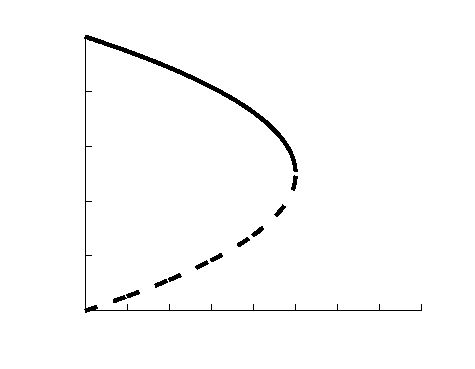
\includegraphics[width={212.50bp},height={161.50bp}]{figures/test}}%
    \gplfronttext
  \end{picture}%
\endgroup

        \caption{Position of the equilibrium points $x^{*}$ vs the parameter $h$}
    \end{figure}

    
    In the plot we see the position of both of the equilibrium points with respect to the value of the parameter $h$. We can see
    that as $h$ increases both points get closer. When $h=0.25$ the points converges together and if $h>0.25$ there are no
    equilibrium points! We say that at $h=0.25$ ocurrs a \emph{bifurcation} and we call the plot of the position of the
    equilibrium points vs the \emph{bifurcation parameter} the \emph{bifurcation diagram}.
    
    
    \section{\sffamily Existence of solutions}

    \begin{thm}{Theorem of \emph{local} existence}{thm:local-ex}
        Assume the function $f(t,x)$ and its partial derivative $(\partial_{x} f)(x,t) = f_{x}(x,t)$ are continuous in a rectangle
        $a<t<b$, $c<x<d$. Then, for any value  $t_0$ and $x_0$ the initial value problem:
        \begin{gather*}
            \begin{cases}
                x'=f(x,t)\\
                x(t_0) = x_0
            \end{cases}
        \end{gather*}
        Has a unique solution valid on some \emph{open} interval $a< \alpha < t< \beta < b$ containing $t_0$
    \end{thm}
    
    When the DE is a linear equation there is a nice propertie:
    \begin{prop}{Existance and uniquiness of a linear equation}{lineq-ex-uniq}
        Consider the IVP:
        \begin{gather*}
            \begin{cases}
                x'+p(t)x=q(t)\\
                x(t_0) = x_0
            \end{cases}
        \end{gather*}
        If $p$ and $q$ are continuous on any open interval $I$ containing $t_0$ then there is a \emph{unique} solution to the
        IVP on the \emph{entire} interval $I$
    \end{prop}
\end{document}
